\documentclass[12pt]{article}

\usepackage{geometry}
\usepackage[utf8]{inputenc}
\usepackage[T2A]{fontenc}
\usepackage[russian]{babel}
\usepackage{graphicx}
\usepackage{caption}
\usepackage{amssymb, gensymb, amsmath}
\usepackage{mathrsfs}
\usepackage{array, colortbl}
\usepackage{multicol}

\title{{\bf Лабораторная работа 5.\, 5. \\ Компьютерная сцинтиляционная $\gamma$-спектрометрия}}
\author{Лось Денис (группа 618)}
\date{21 декабря 2018}

\begin{document}

\maketitle

\paragraph*{Цель работы: } исследовать сцинтиляционные гамма-спектрометры на основе неорганического кристалла NaI и органической сцинтиллирующей пластмассы

\section*{Введение в теоритическую часть}
\par
	Положение пика обратного рассеяния определяется по формуле:
\[
	E_\text{обр} = \frac{E}{1 + 2E / mc^2},
\]
где $E$ --- энергия фотопика.
\par
	Энергетическое разрешение спектрометра
\[
	R_i = \frac{\Delta E_i}{E_i}
\]
, где $\Delta E_i$ --- ширина пика полного поглощения на половине высоты, $E_i$ --- энергия регистрируемого излучения.
\newpage
\section*{Ход работы и результаты исследования}

\subsection*{Построение калибровочного графика}

\begin{table}[h!]
	\centering
	\begin{tabular}{|c|c|}
	\hline
		$N$ канала & $E_i$, МэВ \\
	\hline
		435 & 0.511 \\
	\hline
		1042 & 1.275 \\
	\hline
		553 & 0.662 \\
	\hline
	\end{tabular}
	\caption{Данные для построения калибровочного графика}
\end{table}

\begin{figure}[h!]
	\centering
	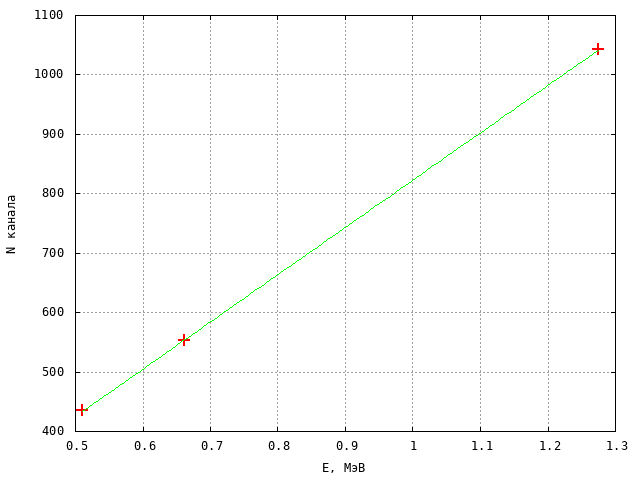
\includegraphics[width = 13cm, height = 7cm]{plot1.png}
	\caption{Калибровочный график $N = a \cdot E_i + b$}
\end{figure}
\par
	Из построенного графика с помощью МНК
\begin{align*}
	a &= \left(795 \pm 3 \right) \, (\text{МэВ})^{-1} \\
	b & = \left(28 \pm 3 \right) \\
\end{align*}
\newpage
\par
	С помощью калибровочного графика определим искомые величины для остальных образцов
\begin{table}[h!]
	\centering
	\begin{tabular}{|c|c|c|c|c|c|}
	\hline
		Источник & $N_i$ & $\Delta N_i$ & $E_i$, МэВ & $\Delta E_i$, МэВ & $R_i$\\
	\hline
	Am	&92	&25&	0.081&	0.031&	0.391 \\
	\hline	
	Co	&956&	63&	1.167&	0.079&	0.068 \\
	\hline	
	Co	&1093&	58&	1.340&	0.073&	0.054 \\
	\hline	
	Eu	&140	&29&	0.141&	0.036&	0.259 \\
	\hline	
	Eu	&228	&40&	0.252&	0.050&	0.200 \\
	\hline	
	Eu	&306	&37&	0.350&	0.047&	0.133 \\
	\hline
	\end{tabular}
\end{table}
\par
	Построим график $R_i^2 = f(1 / E_i)$
\begin{figure}[h!]
	\centering
	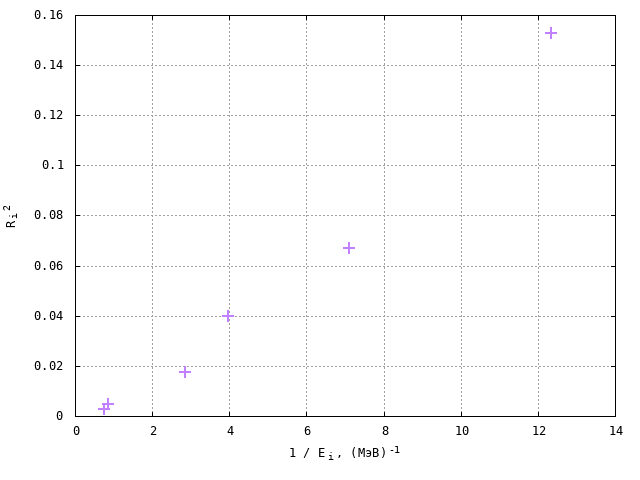
\includegraphics[width = 13cm, height = 7cm]{plot2.png}
\end{figure}
\par
	Произведём измерения для края комптоновского спектра
\begin{table}[h!]
	\centering
	\begin{tabular}{|c|c|c|}
	\hline
		Источник & $N_i$ & $E_\text{ком}$, МэВ\\
	\hline
		Co&	808&	0.981 \\
	\hline
		Cs&	300&	0.342 \\
	\hline
		Na&	264&	0.297 \\
	\hline
	\end{tabular}
\end{table}
\newpage
\par
	Построим график зависимости энергии пика обратного рассеяния от энергии
\begin{figure}[h!]	
	\centering
	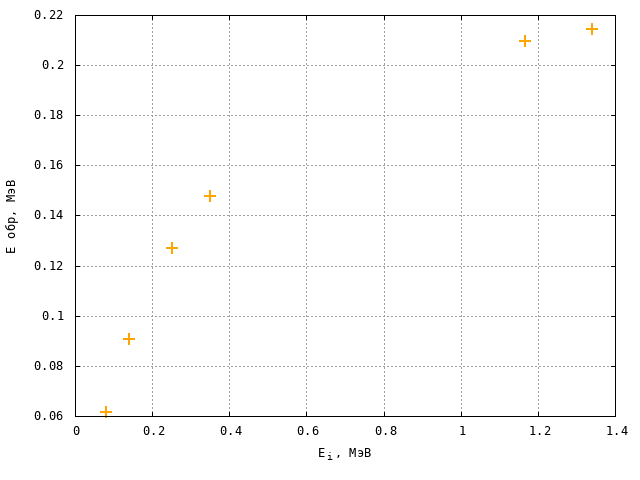
\includegraphics[width = 13cm, height=7cm]{plot3.png}
\end{figure}
\end{document}